
\documentclass[lang=cn,11pt]{elegantpaper}
\usepackage{graphicx}
\usepackage{pythonhighlight}
\usepackage[mathscr]{eucal}
\usepackage{mathrsfs}
\usepackage{booktabs}
\usepackage{capt-of} 





\title{\heiti \LARGE 熵的尝试运用调研报告}
\author{马宇骁~~PB19151769}
\date{\today}



\begin{document}

\maketitle

\begin{abstract}
\noindent \qquad 在上课初接触到熵在数据分析的概念以及做了英雄联盟的实验时候,对此产生兴趣并用Python 编程实践运用,最终使用 \LaTeX{}进行排版展示调研情况。
\keywords{熵,Python,数据分析}
\end{abstract}


\section{熵}

熵(拼音:sh\={a}ng,英语:\lstinline{entropy})泛指某些物质系统状态的一种量度,某些物质系统状态可能出现的程度。亦被社会科学用以借喻人类社会某些状态的程度。  熵的概念是由德国物理学家克劳修斯于1865年所提出。最初是用来描述“能量退化”的物质状态参数之一,在热力学中有广泛的应用。但那时熵仅仅是一个可以通过热量改变来测定的物理量,其本质仍没有很好的解释,直到统计物理、信息论等一系列科学理论发展,熵的本质才逐渐被解释清楚,即,熵的本质是一个系统“内在的混乱程度”。
      
\subsection{熵在信息论中的体现}
在信息论中,随机变量的熵,是变量可能结果中固有的“信息量”、“惊奇度”或“不确定度”的平均水平。即,事件越具确定性,它包含的信息将越少。简言之,信息是不确定度或熵的增加。

1948年,香农将统计物理中熵的概念,引申到信道通信的过程中,从而开创了”信息论“这门学科。香农定义的“熵”又被称为“香农熵”或“信息熵”,即:\\
\begin{equation}
S(p_1,p_2,...,p_n) = -K\sum_{i=1}^{n} p_i log_2 p_i\label{eq:binom}
\end{equation}

其中$i$标记概率空间中所有可能的样本,$p_{i}$表示该样本的出现几率,K是和单位选取相关的任意常数。可以明显看出“信息熵”的定义和“热力学熵”(玻尔兹曼公式)的定义只相差某个比例常数。数学上,可以证明“香农熵”的定义,具有以下良好性质:\\
\textbf{连续性:}

该度量应该是连续的,即,若样本概率值有微小变化,由此引起的熵变化也是微小的。\\
\textbf{极值性:}

当所有样本等几率出现的情况下,熵达到最大值(所有可能的事件等概率时不确定性最高)\\
对于样本等几率分布而言,样本数越大,熵值越大(可能的事件越多,不确定性越高)\\
\textbf{可加性:}

熵的值与过程如何被划分无关。它描述了一个系统与其子系统熵的关系。如果子系统之间的相互作用是已知的,则可以通过子系统的熵来计算一个系统的熵。例如:给定一个有n个样本的均匀分布集合,分为k个箱子(子系统),每个里面有 b1, ..., bk 个样本,合起来的熵应等于系统的熵与各个箱子的熵的和,每个箱子的权重为在该箱中样本的总概率。即,对于正整数bi其中b1 + ... + bk = n来说,
其中S的脚标,标记对应概率空间的样本点个数。事实上,香农证明如果要求度量满足这些性质,则可以完全确定“信息熵”的定义表达式。

\subsection{熵的简单应用作用}
熵的数学表达式简化之后可以表示为:
\begin{equation}
H(X) = -\sum p_i * log_2 p_i\label{eq:binom}
\end{equation}
or
\begin{equation}
Entropy(p) = -\sum_{i=1}^{N} p_i * log_2 p_i\label{eq:binom}
\end{equation}

$f(x)~=~x*log_2(x)$的函数图像如下:
\\~
\begin{center}
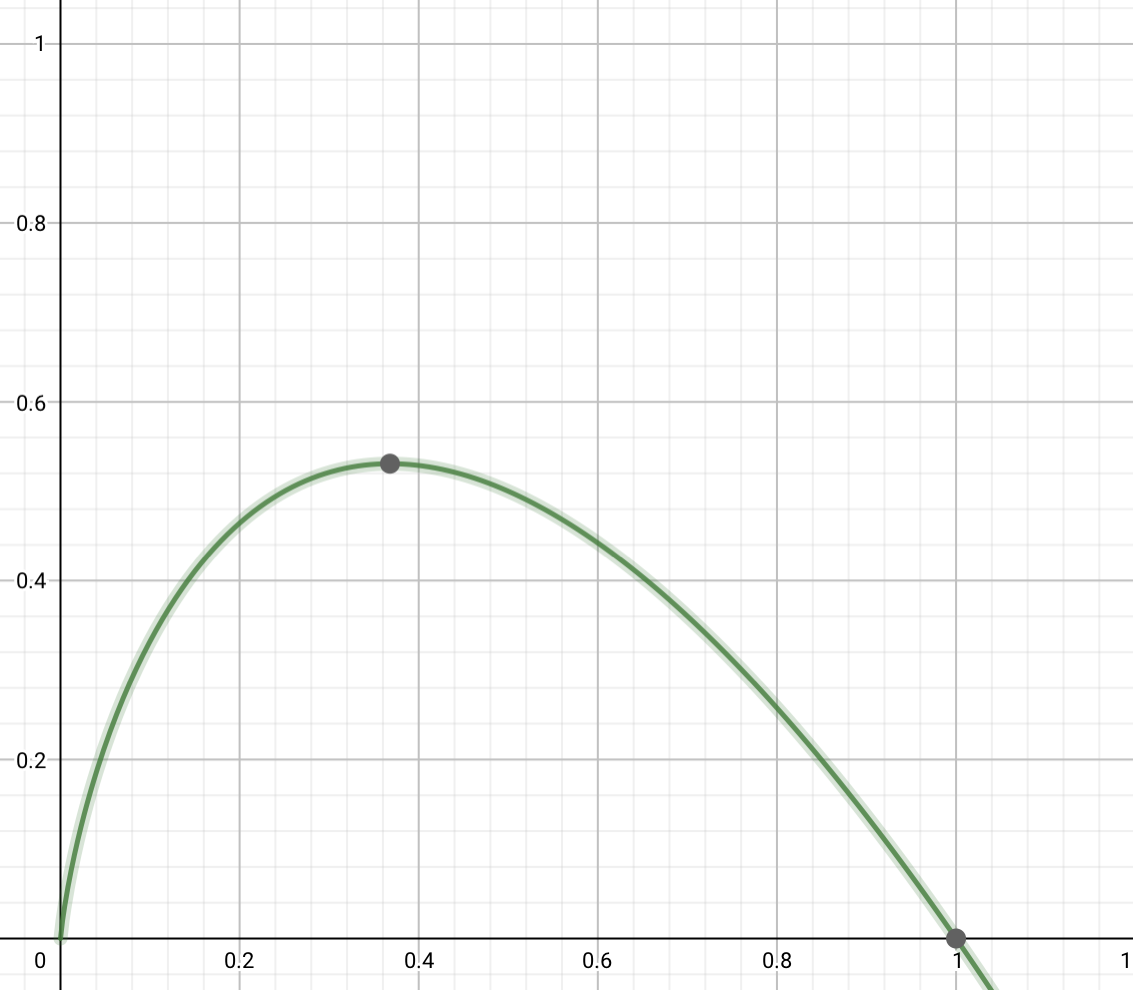
\includegraphics[scale=0.5]{logpic.png}\\
\end{center}

用此公式,考虑到手边现成的80000条英雄联盟实验的数据,因此,选择继续使用该数据集进行简单尝试:

首先,选出所有获胜队伍的所有选手数据(在上一次实验中已经预处理整合完毕),就KDA一项数据进行再次预处理:因为KDA数据为float型不好统计,于是,考虑将原始数据乘以10之后强制转化为整型方便使用count()函数直接统计。
\begin{python}
lolwin = lolplay[lolplay['win']==1]
lolwin['KDA'] = lolwin['KDA']*10
lolwin[['KDA']]=lolwin[['KDA']].astype('int')
ENTRO = []
total = lolwin['index'].count()
for i in range(lolwin['KDA'].max()):
    rate = lolwin[(lolwin['KDA']==i)]['index'].count()/total
    entro = -rate * np.log2(rate)
    ENTRO.append(entro)

HX = float(0)
HX.
for i in ENTRO:
    HX = HX+i
\end{python}

但是,打印HX发现HX的结果为$nan$,与预期不符。经过查看$ENTRO$表发现:
\begin{python}
 0.03689886854299852,
 0.017005118287436182,
 nan,
 0.15591926907688397,
 0.0023304723316794505,
 0.03375045630341993,
 0.05637748574549067,
 0.007379680471335244,
 0.08072092751792367,
 0.05245419737397497,
 0.019063384227767682,
 0.00478956930013355,
 nan,
 0.13850080705066806,
 0.0006211424669610237,
\end{python}

原因应该是部分KDA过小,导致除以$total$的350450的量级时$rate$过于接近0,使得在进行entro运算时以0计算出现结果为$nan$。所以,要在数据基础上对$nan$进行转化使得其在运算中以0的数据在运算中保证结果的正确性。
\begin{python}
WINENTRO =  pd.DataFrame(columns = ['ENTRO'])
WINENTRO['ENTRO'] = ENTRO
#fill all Nan value with zero
WINENTRO['ENTRO']=WINENTRO['ENTRO'].replace(np.nan, 0)

HX = float(0)
for i in WINENTRO['ENTRO']:
    HX = HX+i
\end{python}
最终,$HX$的值为:6.149573322058292;\\
同理,计算出输的一方的KDA的熵为:5.171571388820759。

由此,简单得出一个结论:赢家比输家的KDA更发散,也就是说输家的不确定度/惊奇度更低,战绩更为“平均”一些(平均较差)。

\section{决策树中的熵的应用}
\subsection{总述}
决策树(\lstinline{ Decision Tree})是在已知各种情况发生概率的基础上,通过构成决策树来求取净现值的期望值大于等于零的概率,评价项目风险,判断其可行性的决策分析方法,是直观运用概率分析的一种图解法。由于这种决策分支画成图形很像一棵树的枝干,故称决策树。在机器学习中,决策树是一个预测模型,他代表的是对象属性与对象值之间的一种映射关系。Entropy = 系统的凌乱程度,使用算法ID3, C4.5和C5.0生成树算法使用熵。这一度量是基于信息学理论中熵的概念。

决策树是一种树形结构,其中每个内部节点表示一个属性上的测试,每个分支代表一个测试输出,每个叶节点代表一种类别。\\
\\~
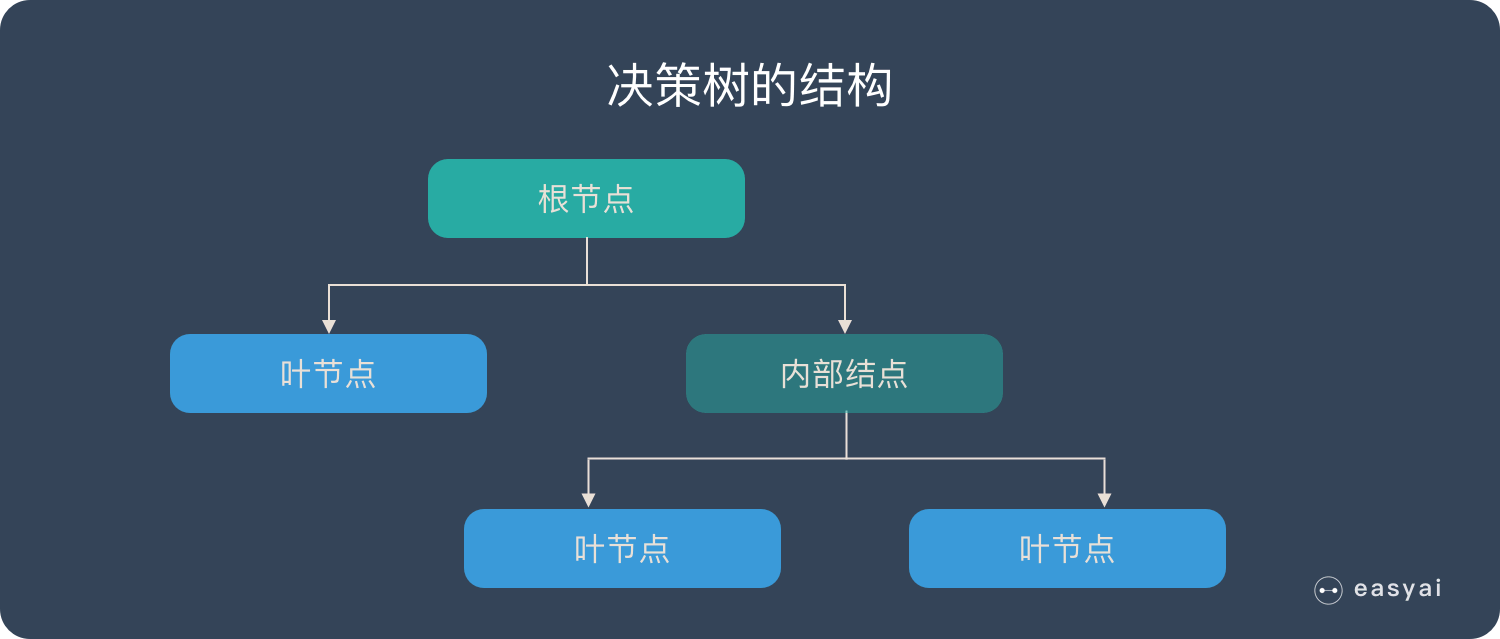
\includegraphics[scale=0.3]{tree.png}\\

在决策树中,损失函数最小化叶子节点中的异质性。因此,目标是选择特征,并在特征中以阈值来构建树,以便在将数据分为两部分时,获得最大可能的同质性,换言之,目标是使树的熵值最小化。

在根节点上,通过香农的熵计算方程式,计算目标列的熵。在分支节点上,为目标列计算加权熵。加权熵意味着每个特征取权重(每个类别的概率)。熵值越小,获得的信息越多。

\subsection{信息增益}
信息增益(\lstinline{Information Gain})即是在数据中观察到的模式,亦即熵的减少。也可以视为父节点的熵减去子节点的熵,计算方式为(1–加权熵)。
\begin{equation}
Gain(D,a) = Entropy(D) - \sum_{k = 1}^{V} \frac{\lvert D^v \rvert}{\lvert D \rvert} Entropy(D^v)   \label{eq:binom}
\end{equation}

\subsection{增益率}
增益率(\lstinline{gain ratio})定义如下:
\begin{equation}
Gain\_ ratio(D,a) = \frac{Gain(D,a)}{IV(a)} \label{eq:binom}
\end{equation}
其中
\begin{equation}
IV(a) = -\sum_{v = 1}^{V} \frac{\lvert D^v \rvert}{\lvert D \rvert} log_2 \frac{\lvert D^v \rvert}{\lvert D \rvert}  \label{eq:binom}
\end{equation}\\
称为属性$a$的“固有值”(\lstinline{intrinsic value})。属性$a$的可能取值数目越多(即V越大),则IV(a)的值通常越大。

\subsection{基尼指数}
基尼指数(\lstinline{Gini不纯度})表示在样本集合中一个随机选中的样本被分错的概率。
注意:Gini指数越小表示集合中被选中的样本被参错的概率越小,也就是说集合的纯度越高,反之,集合越不纯。当集合中所有样本为一个类时,基尼指数为0。

数据集D的纯度基尼值的定义如下:
\begin{equation}
Gini(D) = \sum_{k = 1}^{|y|} \sum_{k' \neq k} p_k p_{k'} = 1 - \sum_{k = 1}^{|y|} {p_k}^2   \label{eq:binom}
\end{equation}

属性$a$的基尼指数定义为:
\begin{equation}
Gini\_ index(D,a) = \sum_{v = 1}^{V}  \frac{\lvert D^v \rvert}{\lvert D \rvert} Gini(D^v)   \label{eq:binom}
\end{equation}

\subsection{单因素划分}
在所给数据集中,将数据根据是否拿到一血,是否拿到一塔,是否拿下第一个小龙,是否先拿下峡谷先锋,是否拿下第一个男爵,是否率先拿下高地塔,最终是否取胜进行分割。
先由单重分类标准对胜负影响根据顺序决策树一共6种:

用Python简单写函数简化计算步骤:\\
\textsc{Python}程序显示如下:
\begin{python}
def ent(a):
    en = 0
    if a == 0|1:
        en = 0
    else:
        en = -(a*np.log2(a)+(1-a)*np.log2(1-a))
    return en

c = lol[lol[' ']==1]['index'].count()/lol['index'].count()

def gain(en0,a,c):
    g = en0
    for i in range(0,len(a)):
        g = g - a[i]*c[i]
    return g
\end{python}

总的信息熵计算,可以看到共两大类:赢,输。所以$\lvert y \rvert=2$ ,占比分别为 $p_1$ = 0.48171689859709227,$p_2$ =  0.5182831014029077 .\\
带入(3)式得:

$Entropy(D)$ = -($p_1$*$log_2$($p_1$) + $p_2$*$log_2$($p_2$)) = 0.9990352804197677
\\~
\\~
\textbf{一血:}\\
\quad 共有$D^1$和$D^2$两个分支结点的熵如下:

$p_1$ = 0.5605694779785196

$p_2$ = 0.43943052202148036

$p_3$ = 0.3996127839103046

$p_4$ = 0.6003872160896955

$Entropy$($D^1$) = 0.9893884370560095

$Entropy$($D^2$) = 0.970723636863251\\
\quad 所以,带入(4)式,得到一血的信息增益为:

$Gain(D,a)$ = 0.018790716797280838
\\~
\\~
\textbf{一塔:}\\
\quad 共有$D^1$和$D^2$两个分支结点的熵如下:

$Entropy$($D^1$) = 0.9099527160549399

$Entropy$($D^2$) = 0.8641293281214248\\
\quad 所以,带入(4)式,得到一塔的信息增益为:

$Gain(D,a)$ = 0.11186678914701398
\\~
\\~
\textbf{一小龙:}\\
\quad 共有$D^1$和$D^2$两个分支结点的熵如下:

同理计算可得:

$Entropy$($D^1$) = 0.9700024072772258

$Entropy$($D^2$) = 0.9506040075800969\\
\quad 所以,带入(4)式,得到一小龙的信息增益为:

$Gain(D,a)$ = 0.039070533722808665
\\~
\\~
\textbf{一峡谷先锋:}\\
\quad 共有$D^1$和$D^2$两个分支结点的熵如下:

同理计算可得:

$Entropy$($D^1$) = 0.9796808347575434

$Entropy$($D^2$) = 0.9640660281983944\\
\quad 所以,带入(4)式,得到一峡谷先锋的信息增益为:

$Gain(D,a)$ = 0.0275286827232073
\\~
\\~
\textbf{一男爵:}\\
\quad 共有$D^1$和$D^2$两个分支结点的熵如下:

同理计算可得:

$Entropy$($D^1$) = 0.6754864921174134

$Entropy$($D^2$) = 0.9095009565004439\\
\quad 所以,带入(4)式,得到一男爵的信息增益为:

$Gain(D,a)$ = 0.16338376176564828
\\~
\\~
\textbf{一高地塔:}\\
\quad 共有$D^1$和$D^2$两个分支结点的熵如下:

同理计算可得:

$Entropy$($D^1$) = 0.46329539348742454

$Entropy$($D^2$) = 0.7097915087139903\\
\quad 所以,带入(4)式,得到一高地塔的信息增益为:

$Gain(D,a)$ = 0.38944181319299565
\\~
\\~
\textbf{小结:}

一般来说,一个属性的信息增益越大,就意味着使用该属性来进行划分所得到的“纯度提升”越大。信息熵越小,数据就越纯,信息增益就越大。对比得出,一高地塔的信息增益最大。因此它被选为划分属性(即作为第一层划分)。分为两类:team1拿到一高地塔和team2拿到一高地塔,前者占总样本数70639的0.40648933308795426,team1胜率为 90.3$ \% $;后者0.5935106669120458,team1的胜率为19.3$\%$。在这里,我来约定,一个集合中的一个team的胜率~$\geq$ 95$ \% $就认为该集合“纯净”(即Gini指数小于等于0.09500000000000003)。

\subsection{双因素划分}
对一高地塔的决策树进行进一步划分,考虑每一个集合都会被划分为两类,最终,每一种划分都会得到4个分支结点。分别记为$D^1$,$D^2$,$D^3$和$D^4$。总熵依旧保持不变:

$Entropy(D)$  = 0.9990352804197677。

于是,对于新的分割再次使用Python编辑函数简化分割运算:\\
\textsc{Python}程序显示如下:
\begin{python}
def gain(en0,a,c):
    g = en0
    for i in range(0,4):
        g = g - a[i]*c[i]
    return g
e0 = 0.9990352804197677
g = gain(e0,e,c)
print(g)
\end{python}
\textbf{一血:}\\
带入(4)式,得到一血的信息增益为:

$Gain(D,a)$ = 0.3973375783126668
\\~
\\~
\textbf{一塔:}\\
带入(4)式,得到一塔的信息增益为:

$Gain(D,a)$ = 0.42783048133276613
\\~
\\~
\textbf{一小龙:}\\
带入(4)式,得到一小龙的信息增益为:

$Gain(D,a)$ = 0.40756669792904987
\\~
\\~
\textbf{一峡谷先锋:}\\
带入(4)式,得到一峡谷先锋的信息增益为:

$Gain(D,a)$ = 0.39559840053492157
\\~
\\~
\textbf{一男爵:}\\
带入(4)式,得到一男爵的信息增益为:

$Gain(D,a)$ = 0.419834851313597
\\~
\\~
\textbf{双因素最终信息增益:}

其中,一塔的信息增益最大,但相比全部数据,一男爵和一塔的差距不大,因此它被选为划分属性(即作为第二层划分)。所以,选择两者的Gini指数计算两种分类方式之后数据的纯度。

将数据带入(7)和(8)式得到结果:

$Gini$\_$index(D,$一男爵) = 0.24300033340652785

$Gini$\_$index(D,$一塔) = 0.2404856305683866

故,一塔的划分会使得结果更纯。\\
\textbf{小结:}

经过再次计算,发现,拿到一高地塔和一塔的胜率为 91.14$ \% $,占总样本数的 28.95$ \% $;拿到一高地塔丢掉一塔的胜率为 87.81$ \% $,占总样本数的 11.69$ \% $;丢掉一高地塔拿到一塔的胜率为 35.36$ \% $,占总样本数的 21.32$ \% $;丢掉一高地塔和一塔的胜率为 10.45$ \% $,占总样本数的 38.03$ \% $。故,现有的4个叶子结点均还未达到纯净,都还需要继续分割。

\subsection{三因素划分}
对一高地塔一塔的决策树进行进一步划分,考虑每一个集合都会被划分为两类,最终,每一种划分都会得到8个分支结点。分别记为$D^1$,$D^2$,$D^3$,$D^4$,$D^5$,$D^6$,$D^7$和$D^8$。总熵依旧保持不变:

$Entropy(D)$  = 0.9990352804197677。

计算过程类似于单因素和双因素,省略过程最终结果如下:
\\~
\\~
\textbf{三因素最终信息增益:}

一血:0.4314506756733847

一小龙:0.4407602480484569

一峡谷先锋:0.4280300414447142

一男爵:0.46003476068898164

其中,一男爵的信息增益明显最大,因此它被选为划分属性(即作为第三层划分)。再分为两类:team1拿到一男爵和team2拿到一男爵,下面在小结中我们看看信息划分的纯净程度。\\
\\~
\textbf{小结:}

经过再次计算,发现,一高地塔+一塔+一男爵的胜率为 94.08$ \% $,占总样本数的 16.39$ \% $;一高地塔+一塔 - 一男爵的胜率为 87.31$ \% $,占总样本数的 12.59$ \% $;一高地塔 - 一塔+一男爵的胜率为 91.80$ \% $,占总样本数的 7.58$ \% $;一高地塔 - 一塔 - 一男爵的胜率为 80.47$ \% $,占总样本数的 4.12$ \% $; - 一高地塔+一塔+一男爵的胜率为 54.28$ \% $,占总样本数的 3.52$ \% $; - 一高地塔+一塔 - 一男爵的胜率为 31.62$ \% $,占总样本数的 17.80$ \% $; - 一高地塔 - 一塔+一男爵的胜率为 41.00$ \% $,占总样本数的 4.09$ \% $; - 一高地塔 - 一塔 - 一男爵的胜率为 6.77$ \% $,占总样本数的 33.94$ \% $。

可以看到,部分数据分割集已经接近设想中的纯净数据集,考虑继续分割。

\subsection{四因素划分}

对一高地塔一塔一男爵的决策树进行进一步划分,考虑每一个集合都会被划分为两类,最终,每一种划分都会得到16个分支结点。分别记为$D^1$,$D^2$,$D^3$,$D^4$,$D^5$,$D^6$,$D^7$,$D^8$,$D^9$,$D^{10}$,$D^{11}$,$D^{12}$,$D^{13}$,$D^{14}$,$D^{15}$和$D^{16}$。总熵依旧保持不变:

$Entropy(D)$  = 0.9990352804197677。

计算过程类似于单因素,双因素和三因素,省略过程最终结果如下:
\\~
\\~
\textbf{四因素最终信息增益:}

一血:0.46360823568055204

一小龙:0.47218757379223314

一峡谷先锋:0.46028469462385696

经由对比,一小龙的信息增益最大,但是信息增益之间差距非常小。考虑到决策树分解到该层不同数据集之间数目差异巨大。信息增益准则对可取数目较多的属性有所偏好,为减少这种偏好带来的不利影响,考虑使用C4.5决策树算法[\lstinline{Quinlan,1993}]不直接使用信息增益。因此,使用增益率进行比较。
\\~
将数据带入(5),(6)式可以得到:

IV(一血) = 3.5764911204937726

IV(一峡谷先锋) = 3.4787793520107853

IV(一小龙) = 3.5716908184116143
\\~
\\~
带回(5)式得到:

Gain$\_$ ratio(D,一血) = 0.1296265585629487

Gain$\_$ ratio(D,一峡谷先锋) = 0.13231212676877757

Gain$\_$ ratio(D,一小龙) = 0.13220281312093587

差距还是很细微,且一峡谷先锋效用最好,因此再考虑Gini指数的差异:

$Gini$\_$index(D,$一血) = 0.22588382501995344

$Gini$\_$index(D,$一小龙) = 0.2220556525751658

$Gini$\_$index(D,$一峡谷先锋) = 0.22748489863231763

看到,3种评估方式中选择一小龙作为划分标准会使得数据集更纯。

因此一小龙被选为划分属性(即作为第四层划分)。再分为两类:team1拿到一小龙和team2拿到一小龙,下面在小结中我们看看信息划分的team1胜率分布程度。\\
\\~
\textbf{小结:}
\begin{table}[htbp]
\begin{center}
\begin{tabular}{cccccc}
\toprule
一高地塔& 一塔& 一男爵& 一小龙& team1胜率 / $ \% $ & 样本占比 / $ \% $\\
\midrule
0&0&0&0&4.66&22.15\\
\hline
0&0&0&1&10.73&11.78\\
\hline
0&0&1&0&35.55&2.21\\
\hline
0&0&1&1&47.40&1.88\\
\hline
0&1&0&0&21.39&9.03\\
\hline
0&1&0&1&42.15&8.77\\
\hline
0&1&1&0&47.17&1.62\\
\hline
0&1&1&1&60.37&1.90\\
\hline
1&0&0&0&76.61&1.96\\
\hline
1&0&0&1&83.97&2.16\\
\hline
1&0&1&0&90.82&3.55\\
\hline
1&0&1&1&92.66&4.03\\
\hline
1&1&0&0&82.55&4.83\\
\hline
1&1&0&1&90.27&7.76\\
\hline
1&1&1&0&92.56&6.40\\
\hline
1&1&1&1&95.05&9.97\\
\bottomrule
\end{tabular}
\caption{四层决策树 \label{tab:reg}}
\end{center}
\end{table}

根据表1,可以看到,终于出现了“纯净”数据集!!!它们是:\textbf{一高地塔一塔一男爵一小龙全部丢掉的集合}和\textbf{一高地塔一塔一男爵一小龙全部拿到的集合}!

因此,在后续决策树延展时只需对剩余的14个叶子结点继续划分提高信息增益。
用Python简单处理为:
\begin{python}
lol = lolfi[(lolfi['team1_firstInhibitor']==i) & (lolfi['team1_firstTower']==j) & (lolfi['team1_firstBaron']==k) & (lolfi['team1_firstDragon']== l)]
if ((i==0) & (j==0) & (k==0) & (l == 0)):
    first_blood_win = 0
    first_riftherald_win = 0
    first_blood_lose = 0
    first_riftherald_lose = 0
elif ((i==1) & (j==1) & (k==1) & (l == 1)):
    first_blood_win = 1
    first_riftherald_win = 1
    first_blood_lose = 1
    first_riftherald_lose = 1
else:
    first_blood_win = lol[(lol['team1_win']==1) & (lol['team1_firstBlood']== 1)]['index'].count()/lol[lol['team1_firstBlood']==1]['index'].count()
    first_riftherald_win = lol[(lol['team1_win']==1) & (lol['team1_firstRiftHerald']== 1)]['index'].count()/lol[lol['team1_firstRiftHerald']==1]['index'].count()
    first_blood_lose = lol[(lol['team1_win']==1) & (lol['team1_firstBlood']== 0)]['index'].count()/lol[lol['team1_firstBlood']==0]['index'].count()
    first_riftherald_lose = lol[(lol['team1_win']==1) & (lol['team1_firstRiftHerald']== 0)]['index'].count()/lol[lol['team1_firstRiftHerald']==0]['index'].count()
\end{python}
\subsection{五因素划分}
对一高地塔一塔一男爵一小龙的决策树进行进一步划分,考虑到已经有两个数据集纯净,剩余14个数据集将被分为28个。
\\~
\textbf{信息增益如下:}

一血:0.563271940227746

一峡谷先锋:0.5611687801713251
\\~
\\~
\textbf{增益率如下:}
将数据带入(5),(6)式可以得到:

IV(一血) = 4.53695623715883

IV(一峡谷先锋) = 4.443879311975698
\\~
\\~
带回(5)式得到:

Gain$\_$ ratio(D,一血) = 0.1241519447806009

Gain$\_$ ratio(D,一峡谷先锋) = 0.12627903252436348
\\~
\\~
\textbf{增益率如下:}

带入(7),(8)顺手一算Gini指数:

$Gini$\_$index(D,$一血) = 0.19163263043136314

$Gini$\_$index(D,$一峡谷先锋) = 0.19277869017200383
\\~

其中,3种指标中只有增益率显示选择一峡谷先锋优于选择一血。故,还是选择一血作为第五层的划分标准。
\\~
\\~
\textbf{小结:}
\begin{table}[htbp]
\begin{center}
\begin{tabular}{ccccccc}
\toprule
一高地塔& 一塔& 一男爵& 一小龙& 一血& team1胜率 / $ \% $ & 样本占比 / $ \% $\\
\midrule
 0 & 0 & 0 & 0 & 0 & 0.00 & 14.18 \\
\hline
 0 & 0 & 0 & 0 & 1 & 0.00 & 7.97 \\
\hline
 0 & 0 & 0 & 1 & 0 & 9.16 & 6.63 \\
\hline
 0 & 0 & 0 & 1 & 1 & 12.74 & 5.15 \\
\hline
 0 & 0 & 1 & 0 & 0 & 35.19	& 1.30 \\
\hline
 0 & 0 & 1 & 0 & 1 & 36.07	& 0.91 \\
\hline
 0 & 0 & 1 & 1 & 0 & 45.15	& 0.93 \\
\hline
 0 & 0 & 1 & 1 & 1 & 49.63	& 0.95 \\
\hline
 0 & 1 & 0 & 0 & 0 & 17.43	& 4.34 \\
\hline
 0 & 1 & 0 & 0 & 1 & 25.06	& 4.69 \\
\hline
 0 & 1 & 0 & 1 & 0 & 33.57	& 3.44 \\
\hline
 0 & 1 & 0 & 1 & 1 & 47.69	& 5.33 \\
\hline
 0 & 1 & 1 & 0 & 0 & 48.28	& 0.74 \\
\hline
 0 & 1 & 1 & 0 & 1 & 46.23	& 0.88 \\
\hline
 0 & 1 & 1 & 1 & 0 & 55.71	& 0.69 \\
\hline
 0 & 1 & 1 & 1 & 1 & 63.06	& 1.2 \\
\hline
 1 & 0 & 0 & 0 & 0 & 76.34	& 1.08 \\
\hline
 1 & 0 & 0 & 0 & 1 & 76.95	& 0.87 \\
\hline
 1 & 0 & 0 & 1 & 0 & 83.29	& 1.04 \\
\hline
 1 & 0 & 0 & 1 & 1 & 84.6	& 1.12 \\
\hline
 1 & 0 & 1 & 0 & 0 & 90.83	& 1.95 \\
\hline
 1 & 0 & 1 & 0 & 1 & 90.8	& 1.6 \\
\hline
 1 & 0 & 1 & 1 & 0 & 92.77	& 1.9 \\
\hline
 1 & 0 & 1 & 1 & 1 & 92.56	& 2.13 \\
\hline
 1 & 1 & 0 & 0 & 0 & 79.92	& 2.07 \\
\hline
 1 & 1 & 0 & 0 & 1 & 84.53	& 2.75 \\
\hline
 1 & 1 & 0 & 1 & 0 & 88.29	& 2.6 \\
\hline
 1 & 1 & 0 & 1 & 1 & 91.27	& 5.16 \\
\hline
 1 & 1 & 1 & 0 & 0 & 92.08	& 2.7 \\
\hline
 1 & 1 & 1 & 0 & 1 & 92.92	& 3.7\\
\hline
 1 & 1 & 1 & 1 & 0 & 100	& 3.39 \\
\hline
 1 & 1 & 1 & 1 & 1 & 100	& 6.58 \\
\bottomrule
\end{tabular}
\caption{五层决策树 \label{tab:reg}}
\end{center}
\end{table}

可以由下方表2看出,靠近两头的数据集越来越“纯净”。最后将一峡谷先锋作为下一次分化的条件。
\subsection{六因素划分}
简单算一下整体Gini指数:

0.19142189882795452

发现已经较小,说明数据纯度已经在一步一步的决策树延伸中加强。

受 \LaTeX{}做大型表格的限制,考虑将胜率以及比率放在图中展示:
\\~
\begin{center}
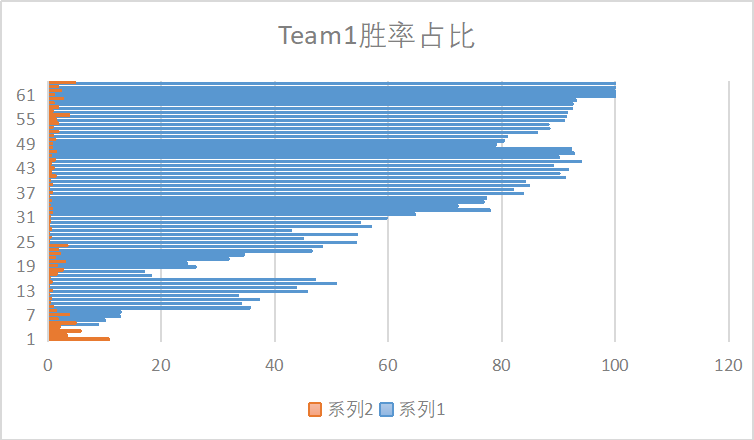
\includegraphics{图片1.png}\\
\end{center}

但这次划分并不能得到十分纯净的数据集。因此如果要考虑进一步纯化,可以将KDA的分段区间作为指标进一步划分。但限于调研学习目的暂不做进一步继续划分。

\section{熵的应用总结}
根据自己的应用和查阅相关信息:信息增益和信息增益率通常用于离散型的特征划分,ID3和C4.5通常情况下都是多叉树,也就是根据离散特征的取值会将数据分到多个子树中;而CART树为二叉树,使用基尼指数作为划分准则,对于离散型特征和连续行特征都能很好的处理。

对每种方法其缺点如下:
\subsection{信息增益}
通过信息增益来选择特征会偏好取值较多的特征,极端情况的例子如果对于某个特征所有样本在此特征上的取值都不相同,这样通过特征计算得到的信息增益式最大的,计算一下 Entropy($D^v$) 是等于0的。
\subsection{增益率}
信息增益率朝着信息增益相反的方向发展,偏好于取值较少的特征。
\subsection{基尼指数}
只能进行二值处理,对于数据分类不止两类的情况分类会遇到困难。
\subsection{实验过程中的小延伸}
在决策树计算过程中总是出现信息增益和基尼指数趋势相同的情况,因此,大胆假设,这两个算法可能是等价的

因此,经过搜索进一步调研借用CSDN夏风之羽的研究决策树算法中基尼指数与信息增益的比较可以看出:
\begin{center}
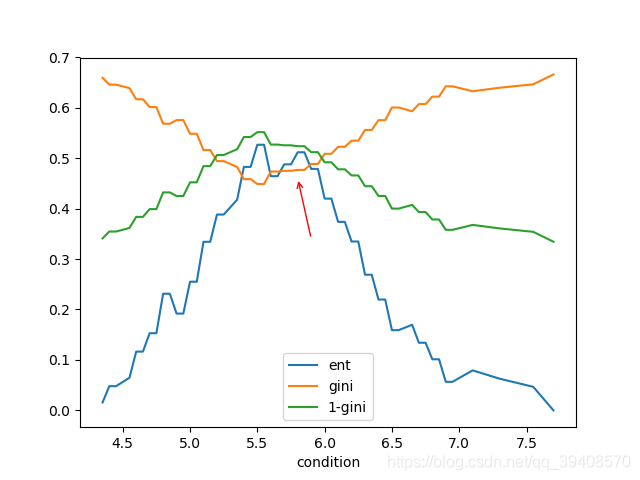
\includegraphics[scale=0.5]{pic2.png}\\
\end{center}

我们想找的反例就是信息增益认为划分A比划分B好,但基尼指数却得到相反的结论。

从图中我们可看到,大体上两种标准的趋势是一样的。似乎只要将它们进行y轴上的放缩,就能得到一个不错的拟合。但实际上,如红色箭头标注的那样,两种标准不是完全一致的。信息增益的同时,基尼指数却没有明显提升。可见,它们不是等价的。

经过不断地试探,他找到了一组合适的反例:
\begin{center}
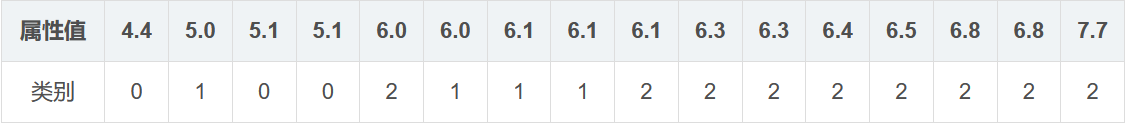
\includegraphics[scale=0.4]{pic3.png}\\
\end{center}

记原始数据集 $D$ 的信息熵为$E_0$​

现在考虑两个划分:

${D_v}_1$​ :属性值 $\le$ 5.55 和 $\textgreater$ 5.55,相应的信息增益记为 $E_1$ ​,基尼指数为 $G_1$

${D_v}_2$ :属性值 $\le$ 6.2 和 $\textgreater$ 6.2 ,相应的信息增益记为 $E_2$​,基尼指数为 $G_2$

经过计算得到:

$E_{0}$ = 1.41973671

$E_{1}$ = 0.60845859, \quad $G_{1}$ = 0.375

$E_{2}$ = 0.55883437, \quad $G_{2}$=0.36111111 

而且 $E_{1}$​是所有划分中信息增益的最大值,$ G_{2}$​是所有划分中基尼指数的最小值.
这就是我们想要的反例:按信息增益,划分${D_v}_1$​优于${D_v}_2$,但按基尼指数${D_v}_2$优于${D_v}_1$​,同时它们都是划分集里的极值,以此形成的id3树和cart树将会不同。

总之,当集合越是混乱的时候,基尼系数对这种趋势的表现越不够充分。相比之下,信息熵则更能区分出混乱和更混乱。\\
\textbf{结论}

    1、信息增益和基尼指数不是等价的

    2、大多数时候它们的区别很小

    3、信息增益对较混乱的集合有很好的表现力,但是基尼指数有所欠缺。另一方面,这也说明较纯的集合,基尼指数可能会区分得更清楚


\section{参考文献}

\begin{lstlisting}
    @article{李鑫宇0信息熵的来源与应用,
  title={信息熵的来源与应用},
  author={李鑫宇},
  journal={文理导航 教育研究与实践},
}

@article{决策树算法中基尼指数与信息增益的比较,
  title={决策树算法中基尼指数与信息增益的比较},
  author={夏风之羽},
  journal={CSDN},
}

@article{2006Inequality,
  title={Inequality Analysis: The Gini Index},
  author={ Liberati, P.  and  Bellu, L. },
  year={2006},
}

@article{机器学习之决策树算法中:信息熵、信息增益、信息增益率和基尼指数的计算,
  title={机器学习之决策树算法中:信息熵、信息增益、信息增益率和基尼指数的计算},
  author={霈行千里},
  journal={CSDN},
}

@article{王兆红2006基于信息熵的决策树,
  title={基于信息熵的决策树},
  author={王兆红},
  journal={潍坊学院学报},
  volume={006},
  number={004},
  pages={28-29},
  year={2006},

  (受限于能力,调试数小时无能现实文献,故附上源码)
}
\end{lstlisting}

\end{document}
